\chapter{Discolog approach} % Main chapter title

\label{Chapter 4} % For referencing the chapter elsewhere, use \ref{Chapter1} 

\lhead{Chapter 4. \emph{Discologapproach}}

%In this section, we introduce our solution for plan recovery in reactive HTN. We also %present the description of the main procedures of plan recovery algorithm.

 In this section, we introduce the Discolog system, a reactive HTN planning, execution, and plan-repairing system. Discolog is a   hybrid system that integrates  a reasoning engine modeled by STRIPS planner to a reactive HTN.
 Discolog uses reactive HTN style to achieve a goal.
 Starting from the top level goal, Discolog recursively decomposes tasks until it reaches a set of primitives tasks that can be directelly executed in the real world. 
 Nevertheless, because of procedural definition of reactive HTN domain knowledge which doesn't contain any logical information allowing the planner reasoning about task decomposition and execution. if the HTN faces breakdowns during the execution, it will be unable to backtrack  to find another decomposition that achieves the execution of the task.
 
 
In order to face this problem, Discolog uses a STRIPS planner that propose a plan recovery starting from the current state of the world and using only the partial information available in the domain knowledge of the HTN. In addition, the system extends the definition of certain HTN tasks from procedural definition to a declarative definition to allow STRIPS planner to reason. An overview of the proposed execution and plan repair system is illustrated in Figure ~\ref{fig:archi}   .
	

The plan recovery in Discolog comprises two main procedures. The first one attempts to detect goal candidate and the second invoke the STRIPS planner. these procedures are described in the next sections.
\section{Goal candidates detection}
When  breakdown occurs, the recovery algorithm will  first look over the goal task and its children to find  tasks in the HTN affected by the breakdown, theses tasks are considered as task candidates for the plan recovery. For example, the move\&paint task 
As presented previously, a breakdown occur in a HTN if one of the task condition fail. Thus repairing a task using STRIPS planner is considered as repairing its failed condition. Once, the list of candidate is identified, the prolog STRIPS planner is called to propose a recovery plan.
\section{STRIPS repair planner}
In order to generate a plan STRIPS has to constitute the planning problem to reason about. First  STRIPS constructs its domain knowledge by extracting partial information from the HTN domain knowledge and extends them to declarative definition.The goal state defines one the failed task condition that  the system attempts to replan  and the current observable state is defined as the initial state.

Next, STRIPS tries for each candidate to generate a plan that repair its failed condition. Finally, the best plan is then passed translated to reactive formalism and passed to the HTN to be executed in the current state.

%\section{Description of the algorithm \ref{euclid}}
%
%Let \textit{HTN} be a model of an Hierarchical Task Network with a top level task \textit{Goal} to achieve.To achieve \textit{Goal} Disco proceed as follow:
%
%
%Starting from the top level goal \textit{Goal}, Disco recursively decomposes tasks until it reaches a set of primitives tasks that can be directelly executed in the real world to achieve \textit{Goal}.
%Each task in Disco has a \textit{status(Task)} $\in$ \{Live,Blocked,Done,Failed,Succeed\}.
%\par Before decomposing a non primitive task or executing primitives task, Disco evaluate the precondition of the this task. If the current state holds the preconditions(Task) then status(Task) is updated to Live. otherwise, Status(Task)= Blocked and the HTN execution is blocked.
%The same, after the execution of a primitive task(execution of the grounding script), Disco evaluate its postconditions. If postconditions(Task) are valid in the current state the status(Task) is updated to done or succeed, otherwise status(Task)= failed and the HTN execution become blocked.
%
%
%At the end of the process, Disco(HTN,Goal) returns either Success(Goal is achieved) or failure if Disco faces breakdown. These breakdowns are detected if the top level goal is not achieved i.e Status(Goal) != Done and Disco has no decomposition or execution to propose. 
%
%When such breakdown occurs, the recovery algorithm will, first look over the \textit{Goal} and its children to find task candidates which can be repaired from the current state in order to recover from the breakdown. This process is handled by the procedure FindCandidates() described in the Algorithm \ref{euclid}.
% :
%\begin{itemize}
%	\item	If the status of task is neither done nor live then the algorithm will attempts to repair its preconditions
%	\item	If the status of task is failed then its postcondition are not valid and the repair algorithm will attempts to repair these postconditions.
%	\item	if the task is nonprimitive and all its applicability conditions are invalid in the current state then the algorithm will attempts te replan to satisfy one of its applicability condition. 
%\end{itemize}
%
%For example, the moveandpaint task which breakdowns in the execution of the walk task because its precondition "isOpen(door)" is no longer valid in the current state. 
%
%Once, the list of candidate is identified, the prolog STRIPS planner is called for each candidate and the solution with the shorter plan is returned to Disco to be executed in the real world.

	\begin{figure}
		\begin{center}
			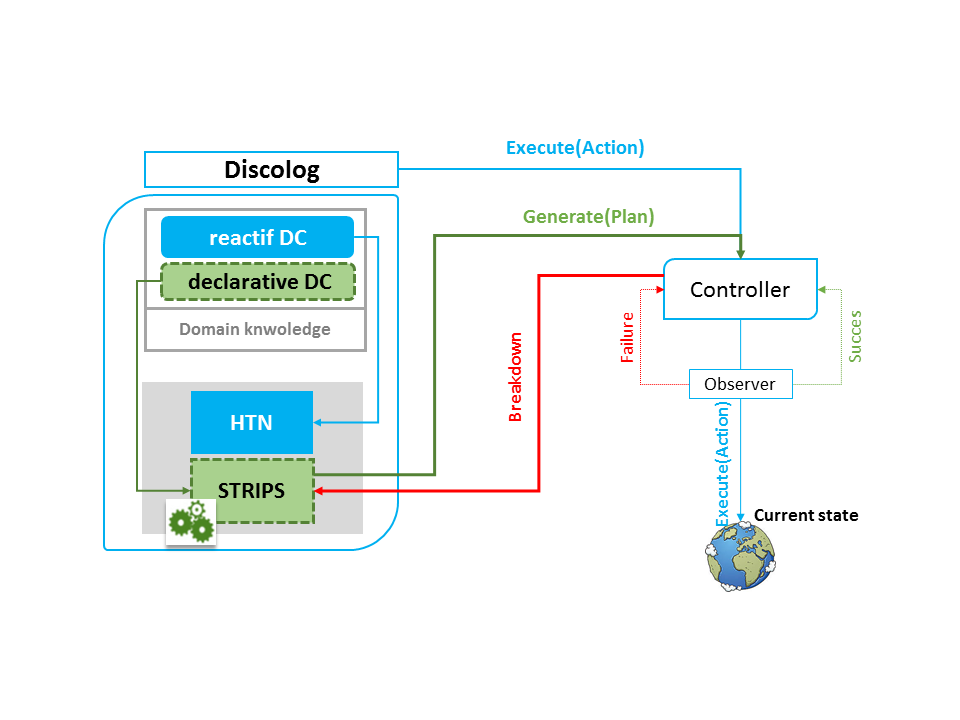
\includegraphics[width=.5\columnwidth]{Pictures/architecture.PNG}
		\end{center}
		\label{fig:archi}
		\caption{High level description of Discolog system}
	\end{figure}